% Disappearing-tracks talk template (Beamer, 16:9, 12pt).
%
% Layout follows the group's earlier approval talk (EXO-19-010): section
% navigation bar in the footer and a
% "Since <last review>" call-out. Adapted for slides built from DisappTrks_Nano
% output; see ../SKILL.md ("Conventions from the previous iteration").
%
% Every placeholder is marked TODO. Nothing here is a result: numbers, figures, and
% author/logo material must come from real outputs or the presenter. Group logos
% are NOT included -- add the approved files yourself (see \titlegraphic below).
%
% Build:  latexmk -pdf -interaction=nonstopmode -halt-on-error -outdir=build talk.tex
% Copy this file into <deck>/, point \graphicspath and \input at your figures/tables.
\documentclass[aspectratio=169,12pt]{beamer}

\usetheme{default}
\usecolortheme{default}
\usepackage{graphicx}
\usepackage{booktabs}
\usepackage{amsmath}
\usepackage{siunitx}
\usepackage{tikz}
\usetikzlibrary{arrows.meta,positioning,calc}
\graphicspath{{figures/}{../figures/}}

% ------------------------------------------------------------------ colors
\definecolor{navbar}{RGB}{23,73,127}      % footer bar
\definecolor{sourcegreen}{RGB}{40,160,40} % source tag
\definecolor{sincered}{RGB}{200,30,30}    % "since last review" box
\setbeamercolor{frametitle}{fg=black,bg=white}
\setbeamerfont{frametitle}{size=\large,series=\bfseries}
\setbeamercolor{section in head/foot}{fg=white,bg=navbar}
\setbeamercolor{title in head/foot}{fg=white,bg=black}
\setbeamercolor{structure}{fg=navbar}
\setbeamertemplate{navigation symbols}{}
\setbeamertemplate{itemize items}[circle]

% ------------------------------------------------------- footer: section nav
% Section names come from \section{...}; the current one is highlighted.
\setbeamertemplate{footline}{%
  \leavevmode\hbox{%
    \begin{beamercolorbox}[wd=.55\paperwidth,ht=3ex,dp=1.2ex,left]{section in head/foot}%
      \hspace*{1em}\insertsectionnavigationhorizontal{.53\paperwidth}{}{}%
    \end{beamercolorbox}%
    \begin{beamercolorbox}[wd=.45\paperwidth,ht=3ex,dp=1.2ex,right]{title in head/foot}%
      \scriptsize
      \insertshorttitle\ \ {\footnotesize\insertframenumber}\hspace*{1em}%
    \end{beamercolorbox}}%
}

% ------------------------------------------------------------------- macros
% One-line takeaway under a figure or table.
\newcommand{\takeaway}[1]{\par\vspace{10pt}\centering\small\textbf{#1}\par}

% "Since <last review stage>" call-out, bottom-right above the footer.
\newcommand{\sincebox}[1]{%
  \begin{tikzpicture}[remember picture,overlay]
    \node[anchor=south east,draw=sincered,text=sincered,align=center,inner sep=4pt,
          font=\small] at ($(current page.south east)+(-0.3cm,1.1cm)$) {#1};
  \end{tikzpicture}}

% Figure that degrades to a labelled placeholder box if the file is missing, so the
% template compiles before any real figures exist. Size by HEIGHT (see hep-slides).
\newcommand{\slidefig}[2][0.66\textheight]{%
  \IfFileExists{#2}{\includegraphics[height=#1]{#2}}%
  {\fbox{\parbox[c][#1][c]{0.45\textwidth}{\centering TODO figure:\\ \texttt{\detokenize{#2}}}}}}

% Table that degrades to a placeholder if the .tex file is missing.
\newcommand{\slidetable}[1]{%
  \IfFileExists{#1}{\input{#1}}%
  {\fbox{TODO table: \texttt{\detokenize{#1}}}}}

% Physics shorthand
\newcommand{\ptmiss}{\ensuremath{p_T^{\mathrm{miss,\,no\,\mu}}}}
\newcommand{\nlayers}{\ensuremath{n_{\mathrm{layers}}}}

% ------------------------------------------------------------------ metadata
\title[Disappearing tracks]{Search for Disappearing Tracks} % TODO title
\subtitle{Talk / meeting name}                              % TODO
\author[Presenter]{Presenter Name}                          % TODO: presenter (bold) then co-authors
\institute[OSU]{The Ohio State University}                  % TODO add collaborating institutions
\date[\today]{\today}
% Group logos: add the approved files, do not fabricate them.
% \titlegraphic{\includegraphics[height=1.2cm]{logo_osu.pdf}}

\begin{document}

\begin{frame}[plain]
  \titlepage
  % TODO if it exists: links to analysis note version, paper draft, review twiki.
\end{frame}

% ===================================================================== Intro
\section{Intro}
\begin{frame}{Signature: a track that vanishes before the outer tracker}
  \begin{itemize}
    \item TODO: signature, signal model, why it is long-lived
    \item Missing outer hits; little calorimeter energy; no muon-chamber hits
  \end{itemize}
  \sincebox{TODO: Since last update: \ldots}
\end{frame}

% ================================================================= Selection
\section{Selection}
\begin{frame}{Basic selection requires an ISR-like event}
  \begin{itemize}
    \item TODO: primary vertex, \ptmiss{} threshold, jet requirements, $\Delta\phi$ vetoes
    \item Read the current values from \texttt{DisappTrks\_Nano}, not from an old talk
  \end{itemize}
\end{frame}

\begin{frame}{Candidate-track selection}
  \centering
  \begin{tabular}{p{0.3\textwidth}p{0.5\textwidth}}
    \toprule
    Requirement & Cut (TODO: from \texttt{search\_track\_mask}) \\
    \midrule
    Kinematics & \ldots \\
    \bottomrule
  \end{tabular}
\end{frame}

% =============================================================== Backgrounds
\section{Backgrounds}
% Per-background arc: method -> systematics -> closure.
\begin{frame}{Method: the estimate is a product of measured probabilities}
  \centering
  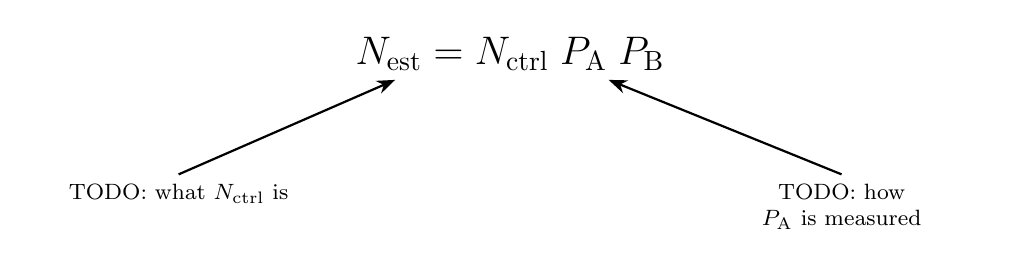
\begin{tikzpicture}[lab/.style={align=center,font=\footnotesize,text width=3.6cm},
                      arr/.style={-{Stealth},thick}]
    % TODO: replace with the real formula and factor descriptions.
    \node (f) {\Large $N_{\mathrm{est}} = N_{\mathrm{ctrl}}\;P_{\mathrm{A}}\;P_{\mathrm{B}}$};
    \node[lab,below left=1.2cm and 0.2cm of f]  (a) {TODO: what $N_{\mathrm{ctrl}}$ is};
    \node[lab,below right=1.2cm and 0.2cm of f] (b) {TODO: how $P_{\mathrm{A}}$ is measured};
    \draw[arr] (a.north) -- ($(f.south west)!0.3!(f.south)$);
    \draw[arr] (b.north) -- ($(f.south)!0.6!(f.south east)$);
  \end{tikzpicture}
\end{frame}

\begin{frame}{Systematics on the estimate: TODO size and origin}
  \begin{itemize}
    \item TODO: each systematic, how it was derived, its size range
  \end{itemize}
\end{frame}

\begin{frame}{Closure: TODO agreement statement}
  \centering
  \slidetable{tables/closure.tex}
  \takeaway{TODO: state agreement, and under which selection it was measured}
\end{frame}

% ==================================================================== Signal
\section{Signal}
\begin{frame}{Signal corrections and systematics}
  \begin{itemize}
    \item TODO: hits, trigger efficiency, ISR; systematics summary table
  \end{itemize}
\end{frame}

% =================================================================== Results
\section{Results}
\begin{frame}{Expected backgrounds: TODO takeaway}
  \centering\footnotesize\renewcommand{\arraystretch}{0.9}
  \slidetable{tables/generated/total_1.tex}
  \takeaway{State uncertainty type (statistical only / stat. + syst.)}
\end{frame}

\begin{frame}{Interpretation: TODO takeaway}
  \centering
  \slidefig{limit_plot.pdf}
\end{frame}

% ================================================================ Conclusion
\section{Conclusion}
\begin{frame}{Summary and next steps}
  \begin{itemize}
    \item TODO: what was done
    \item TODO: what changed since the last review/update
    \item TODO: what is requested / the concrete next steps
  \end{itemize}
\end{frame}

% ==================================================================== Backup
\appendix
\section*{Backup}
\begin{frame}[noframenumbering]{Backup: TODO}
  \centering
  \slidefig{backup_plot.pdf}
\end{frame}

\end{document}
